\section{Controle Modular Local}

\begin{frame}{Composição paralela das subplantas assíncronas.}

    \begin{itemize}
        \item \textbf{Modelagem individual de cada componente;} 
    \end{itemize}

    Plantas com restrições individuais

    \begin{itemize}
        \item \textit{Processing Machine 1}
        \item \textit{Processing Machine 2}
    \end{itemize}

    Ambas restrições são independentes, e ligeiramente diferentes, e comandam o \textbf{ciclo de funcionamento} das \textit{Processing Machines}, que trabalham de forma autônoma ao resto do sistema executam suas respectivas ações - de enchimento com \textit{milkshake} e cobertura - uma vez que o sensor acuse a chegada do copo.


\end{frame}

\begin{frame}{\textit{Processing Machine} (PM1).}

    Restricão para a subplanta composta apenas da \textit{Processing Machine 1}.

    \begin{figure}[htbp]
        \centering
        \resizebox{0.7\textwidth}{!}{


\tikzset{every picture/.style={line width=0.75pt}} %set default line width to 0.75pt        

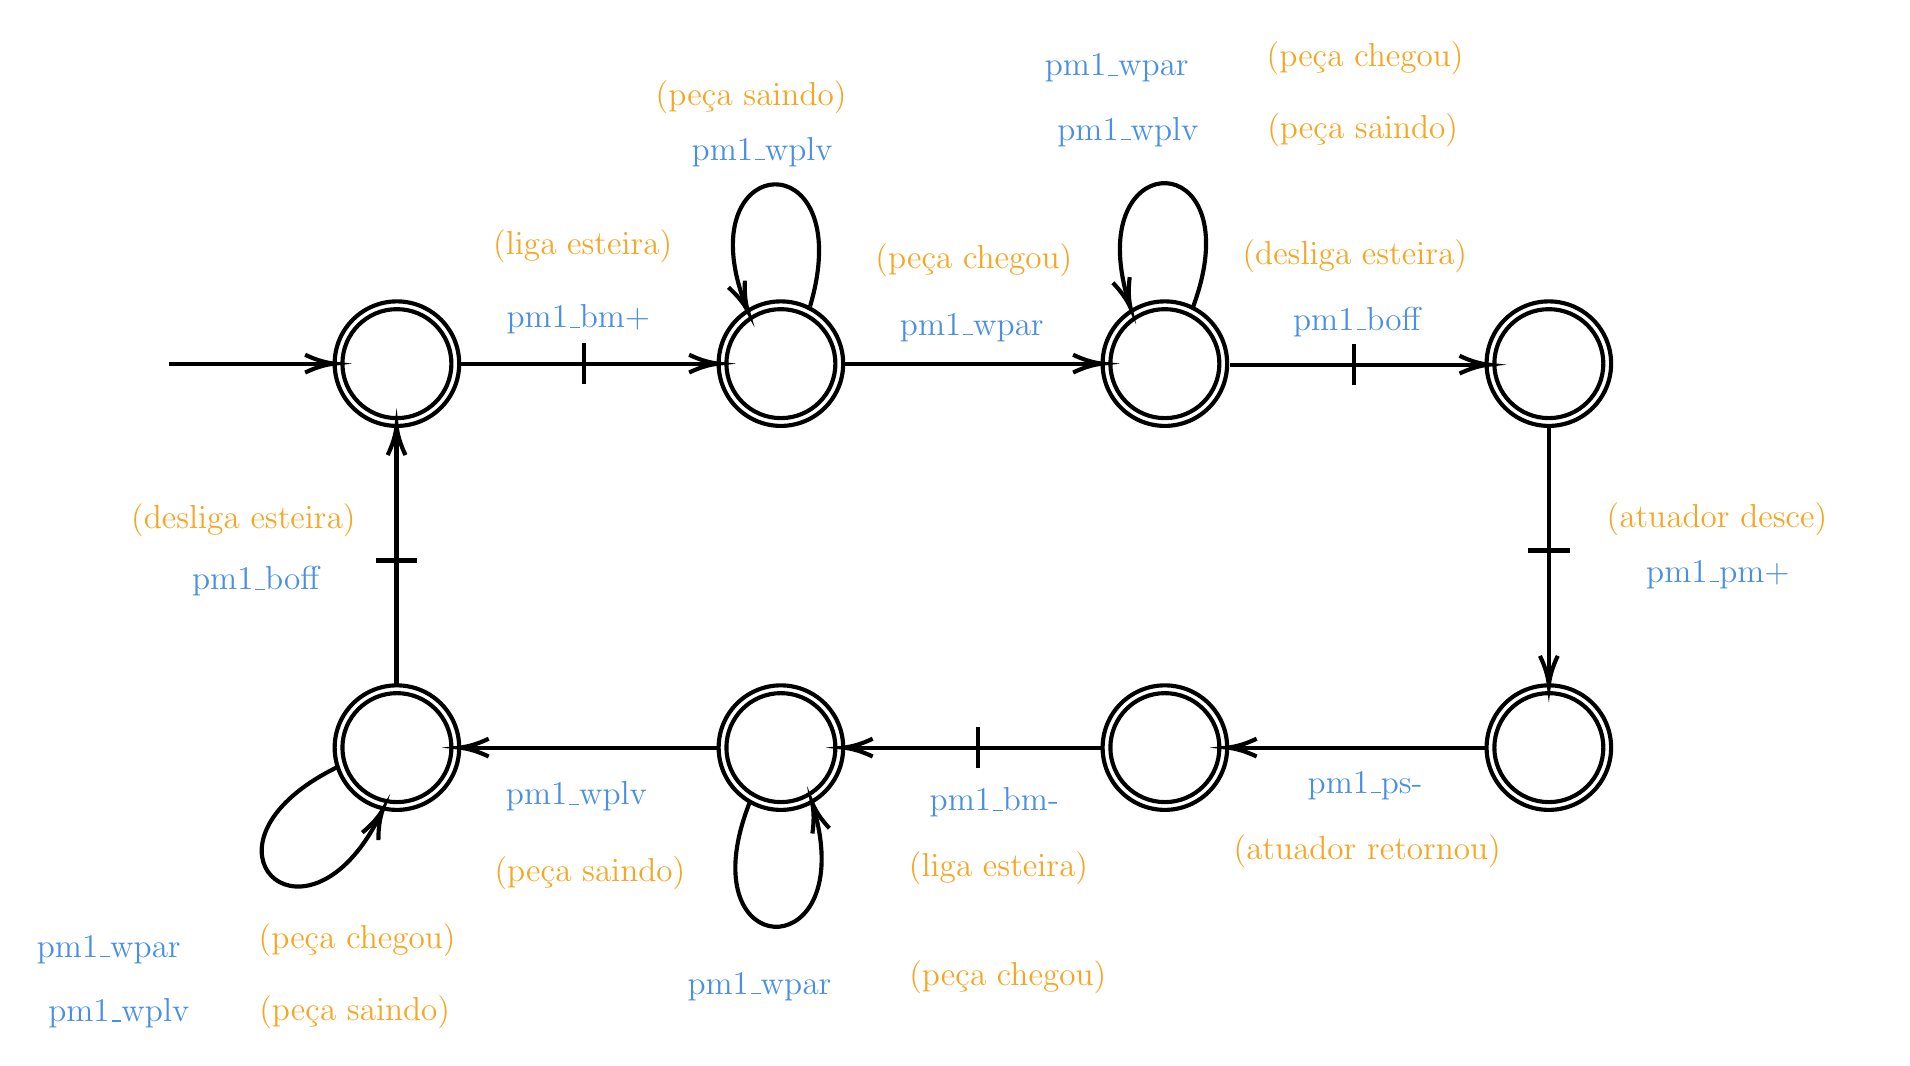
\begin{tikzpicture}[x=0.75pt,y=0.75pt,yscale=-1,xscale=1]
%uncomment if require: \path (0,3420); %set diagram left start at 0, and has height of 3420

%Shape: Circle [id:dp5021231821953818] 
\draw  [line width=1.5]  (1371.5,2916.5) .. controls (1371.5,2899.93) and (1384.93,2886.5) .. (1401.5,2886.5) .. controls (1418.07,2886.5) and (1431.5,2899.93) .. (1431.5,2916.5) .. controls (1431.5,2933.07) and (1418.07,2946.5) .. (1401.5,2946.5) .. controls (1384.93,2946.5) and (1371.5,2933.07) .. (1371.5,2916.5) -- cycle ;
%Shape: Circle [id:dp5289461805073701] 
\draw  [line width=1.5]  (1375.25,2916.5) .. controls (1375.25,2902) and (1387,2890.25) .. (1401.5,2890.25) .. controls (1416,2890.25) and (1427.75,2902) .. (1427.75,2916.5) .. controls (1427.75,2931) and (1416,2942.75) .. (1401.5,2942.75) .. controls (1387,2942.75) and (1375.25,2931) .. (1375.25,2916.5) -- cycle ;
%Straight Lines [id:da4788090574749646] 
\draw [line width=1.5]    (1291.5,2916.5) -- (1368.5,2916.5) ;
\draw [shift={(1371.5,2916.5)}, rotate = 180] [color={rgb, 255:red, 0; green, 0; blue, 0 }  ][line width=1.5]    (14.21,-4.28) .. controls (9.04,-1.82) and (4.3,-0.39) .. (0,0) .. controls (4.3,0.39) and (9.04,1.82) .. (14.21,4.28)   ;
%Straight Lines [id:da8018832314051378] 
\draw [line width=1.5]    (1431.5,2916.5) -- (1454.5,2916.5) -- (1553.5,2916.5) ;
\draw [shift={(1556.5,2916.5)}, rotate = 180] [color={rgb, 255:red, 0; green, 0; blue, 0 }  ][line width=1.5]    (14.21,-4.28) .. controls (9.04,-1.82) and (4.3,-0.39) .. (0,0) .. controls (4.3,0.39) and (9.04,1.82) .. (14.21,4.28)   ;
%Straight Lines [id:da0076803473792970145] 
\draw [line width=1.5]    (1491.5,2906.5) -- (1491.5,2926.5) ;

%Shape: Circle [id:dp22625731925102777] 
\draw  [line width=1.5]  (1556.5,2916.5) .. controls (1556.5,2899.93) and (1569.93,2886.5) .. (1586.5,2886.5) .. controls (1603.07,2886.5) and (1616.5,2899.93) .. (1616.5,2916.5) .. controls (1616.5,2933.07) and (1603.07,2946.5) .. (1586.5,2946.5) .. controls (1569.93,2946.5) and (1556.5,2933.07) .. (1556.5,2916.5) -- cycle ;
%Straight Lines [id:da9270365039391677] 
\draw [line width=1.5]    (1616.5,2916.5) -- (1738.5,2916.5) ;
\draw [shift={(1741.5,2916.5)}, rotate = 180] [color={rgb, 255:red, 0; green, 0; blue, 0 }  ][line width=1.5]    (14.21,-4.28) .. controls (9.04,-1.82) and (4.3,-0.39) .. (0,0) .. controls (4.3,0.39) and (9.04,1.82) .. (14.21,4.28)   ;
%Shape: Circle [id:dp8790830623806889] 
\draw  [line width=1.5]  (1741.5,2916.5) .. controls (1741.5,2899.93) and (1754.93,2886.5) .. (1771.5,2886.5) .. controls (1788.07,2886.5) and (1801.5,2899.93) .. (1801.5,2916.5) .. controls (1801.5,2933.07) and (1788.07,2946.5) .. (1771.5,2946.5) .. controls (1754.93,2946.5) and (1741.5,2933.07) .. (1741.5,2916.5) -- cycle ;
%Shape: Circle [id:dp05996581087867403] 
\draw  [line width=1.5]  (1926.5,2916.5) .. controls (1926.5,2899.93) and (1939.93,2886.5) .. (1956.5,2886.5) .. controls (1973.07,2886.5) and (1986.5,2899.93) .. (1986.5,2916.5) .. controls (1986.5,2933.07) and (1973.07,2946.5) .. (1956.5,2946.5) .. controls (1939.93,2946.5) and (1926.5,2933.07) .. (1926.5,2916.5) -- cycle ;
%Straight Lines [id:da8561532153311397] 
\draw [line width=1.5]    (1956.5,2946.5) -- (1956.5,2969.5) -- (1956.5,3068.5) ;
\draw [shift={(1956.5,3071.5)}, rotate = 270] [color={rgb, 255:red, 0; green, 0; blue, 0 }  ][line width=1.5]    (14.21,-4.28) .. controls (9.04,-1.82) and (4.3,-0.39) .. (0,0) .. controls (4.3,0.39) and (9.04,1.82) .. (14.21,4.28)   ;
%Straight Lines [id:da5406403779740838] 
\draw [line width=1.5]    (1966.5,3006.5) -- (1946.5,3006.5) ;

%Shape: Circle [id:dp1389806805521474] 
\draw  [line width=1.5]  (1926.5,3101.5) .. controls (1926.5,3084.93) and (1939.93,3071.5) .. (1956.5,3071.5) .. controls (1973.07,3071.5) and (1986.5,3084.93) .. (1986.5,3101.5) .. controls (1986.5,3118.07) and (1973.07,3131.5) .. (1956.5,3131.5) .. controls (1939.93,3131.5) and (1926.5,3118.07) .. (1926.5,3101.5) -- cycle ;
%Straight Lines [id:da3566574988633957] 
\draw [line width=1.5]    (1804.5,3101.5) -- (1926.5,3101.5) ;
\draw [shift={(1801.5,3101.5)}, rotate = 0] [color={rgb, 255:red, 0; green, 0; blue, 0 }  ][line width=1.5]    (14.21,-4.28) .. controls (9.04,-1.82) and (4.3,-0.39) .. (0,0) .. controls (4.3,0.39) and (9.04,1.82) .. (14.21,4.28)   ;
%Shape: Circle [id:dp5939143750931828] 
\draw  [line width=1.5]  (1741.5,3101.5) .. controls (1741.5,3084.93) and (1754.93,3071.5) .. (1771.5,3071.5) .. controls (1788.07,3071.5) and (1801.5,3084.93) .. (1801.5,3101.5) .. controls (1801.5,3118.07) and (1788.07,3131.5) .. (1771.5,3131.5) .. controls (1754.93,3131.5) and (1741.5,3118.07) .. (1741.5,3101.5) -- cycle ;
%Shape: Circle [id:dp9635042203289415] 
\draw  [line width=1.5]  (1556.5,3101.5) .. controls (1556.5,3084.93) and (1569.93,3071.5) .. (1586.5,3071.5) .. controls (1603.07,3071.5) and (1616.5,3084.93) .. (1616.5,3101.5) .. controls (1616.5,3118.07) and (1603.07,3131.5) .. (1586.5,3131.5) .. controls (1569.93,3131.5) and (1556.5,3118.07) .. (1556.5,3101.5) -- cycle ;
%Shape: Circle [id:dp022192289610075466] 
\draw  [line width=1.5]  (1371.5,3101.5) .. controls (1371.5,3084.93) and (1384.93,3071.5) .. (1401.5,3071.5) .. controls (1418.07,3071.5) and (1431.5,3084.93) .. (1431.5,3101.5) .. controls (1431.5,3118.07) and (1418.07,3131.5) .. (1401.5,3131.5) .. controls (1384.93,3131.5) and (1371.5,3118.07) .. (1371.5,3101.5) -- cycle ;
%Straight Lines [id:da8665047753384527] 
\draw [line width=1.5]    (1741.5,3101.5) -- (1718.5,3101.5) -- (1619.5,3101.5) ;
\draw [shift={(1616.5,3101.5)}, rotate = 360] [color={rgb, 255:red, 0; green, 0; blue, 0 }  ][line width=1.5]    (14.21,-4.28) .. controls (9.04,-1.82) and (4.3,-0.39) .. (0,0) .. controls (4.3,0.39) and (9.04,1.82) .. (14.21,4.28)   ;
%Straight Lines [id:da33313592666384406] 
\draw [line width=1.5]    (1681.5,3111.5) -- (1681.5,3091.5) ;

%Shape: Circle [id:dp323983994895517] 
\draw  [line width=1.5]  (1560.25,2916.5) .. controls (1560.25,2902) and (1572,2890.25) .. (1586.5,2890.25) .. controls (1601,2890.25) and (1612.75,2902) .. (1612.75,2916.5) .. controls (1612.75,2931) and (1601,2942.75) .. (1586.5,2942.75) .. controls (1572,2942.75) and (1560.25,2931) .. (1560.25,2916.5) -- cycle ;
%Shape: Circle [id:dp061991462662711605] 
\draw  [line width=1.5]  (1745.25,2916.5) .. controls (1745.25,2902) and (1757,2890.25) .. (1771.5,2890.25) .. controls (1786,2890.25) and (1797.75,2902) .. (1797.75,2916.5) .. controls (1797.75,2931) and (1786,2942.75) .. (1771.5,2942.75) .. controls (1757,2942.75) and (1745.25,2931) .. (1745.25,2916.5) -- cycle ;
%Shape: Circle [id:dp8712457883247433] 
\draw  [line width=1.5]  (1930.25,2916.5) .. controls (1930.25,2902) and (1942,2890.25) .. (1956.5,2890.25) .. controls (1971,2890.25) and (1982.75,2902) .. (1982.75,2916.5) .. controls (1982.75,2931) and (1971,2942.75) .. (1956.5,2942.75) .. controls (1942,2942.75) and (1930.25,2931) .. (1930.25,2916.5) -- cycle ;
%Shape: Circle [id:dp4032269267721291] 
\draw  [line width=1.5]  (1930.25,3101.5) .. controls (1930.25,3087) and (1942,3075.25) .. (1956.5,3075.25) .. controls (1971,3075.25) and (1982.75,3087) .. (1982.75,3101.5) .. controls (1982.75,3116) and (1971,3127.75) .. (1956.5,3127.75) .. controls (1942,3127.75) and (1930.25,3116) .. (1930.25,3101.5) -- cycle ;
%Shape: Circle [id:dp7865107563162004] 
\draw  [line width=1.5]  (1745.25,3101.5) .. controls (1745.25,3087) and (1757,3075.25) .. (1771.5,3075.25) .. controls (1786,3075.25) and (1797.75,3087) .. (1797.75,3101.5) .. controls (1797.75,3116) and (1786,3127.75) .. (1771.5,3127.75) .. controls (1757,3127.75) and (1745.25,3116) .. (1745.25,3101.5) -- cycle ;
%Shape: Circle [id:dp6415554207822463] 
\draw  [line width=1.5]  (1560.25,3101.5) .. controls (1560.25,3087) and (1572,3075.25) .. (1586.5,3075.25) .. controls (1601,3075.25) and (1612.75,3087) .. (1612.75,3101.5) .. controls (1612.75,3116) and (1601,3127.75) .. (1586.5,3127.75) .. controls (1572,3127.75) and (1560.25,3116) .. (1560.25,3101.5) -- cycle ;
%Shape: Circle [id:dp25769850815519857] 
\draw  [line width=1.5]  (1375.25,3101.5) .. controls (1375.25,3087) and (1387,3075.25) .. (1401.5,3075.25) .. controls (1416,3075.25) and (1427.75,3087) .. (1427.75,3101.5) .. controls (1427.75,3116) and (1416,3127.75) .. (1401.5,3127.75) .. controls (1387,3127.75) and (1375.25,3116) .. (1375.25,3101.5) -- cycle ;
%Straight Lines [id:da896726859664503] 
\draw [line width=1.5]    (1802.67,2917) -- (1825.67,2917) -- (1924.67,2917) ;
\draw [shift={(1927.67,2917)}, rotate = 180] [color={rgb, 255:red, 0; green, 0; blue, 0 }  ][line width=1.5]    (14.21,-4.28) .. controls (9.04,-1.82) and (4.3,-0.39) .. (0,0) .. controls (4.3,0.39) and (9.04,1.82) .. (14.21,4.28)   ;
%Straight Lines [id:da40191603415797883] 
\draw [line width=1.5]    (1862.67,2907) -- (1862.67,2927) ;

%Straight Lines [id:da303290828710558] 
\draw [line width=1.5]    (1434.5,3101.5) -- (1556.5,3101.5) ;
\draw [shift={(1431.5,3101.5)}, rotate = 0] [color={rgb, 255:red, 0; green, 0; blue, 0 }  ][line width=1.5]    (14.21,-4.28) .. controls (9.04,-1.82) and (4.3,-0.39) .. (0,0) .. controls (4.3,0.39) and (9.04,1.82) .. (14.21,4.28)   ;
%Straight Lines [id:da04070398455869095] 
\draw [line width=1.5]    (1401.33,3071.33) -- (1401.33,3048.33) -- (1401.33,2949.33) ;
\draw [shift={(1401.33,2946.33)}, rotate = 90] [color={rgb, 255:red, 0; green, 0; blue, 0 }  ][line width=1.5]    (14.21,-4.28) .. controls (9.04,-1.82) and (4.3,-0.39) .. (0,0) .. controls (4.3,0.39) and (9.04,1.82) .. (14.21,4.28)   ;
%Straight Lines [id:da6773677195850383] 
\draw [line width=1.5]    (1391.33,3011.33) -- (1411.33,3011.33) ;

%Shape: Boxed Bezier Curve [id:dp5167110010811578] 
\draw [line width=1.5]    (1600.54,2888.94) .. controls (1622.83,2813.24) and (1551.33,2813.02) .. (1565.15,2874.31) .. controls (1566.15,2878.74) and (1567.59,2883.49) .. (1569.55,2888.56) ;
\draw [shift={(1570.63,2891.27)}, rotate = 247.54] [color={rgb, 255:red, 0; green, 0; blue, 0 }  ][line width=1.5]    (14.21,-4.28) .. controls (9.04,-1.82) and (4.3,-0.39) .. (0,0) .. controls (4.3,0.39) and (9.04,1.82) .. (14.21,4.28)   ;
%Shape: Boxed Bezier Curve [id:dp9243950747298513] 
\draw [line width=1.5]    (1784.98,2889.43) .. controls (1812.53,2815.49) and (1741.22,2810.25) .. (1750.7,2872.35) .. controls (1751.38,2876.84) and (1752.49,2881.68) .. (1754.09,2886.87) ;
\draw [shift={(1754.98,2889.66)}, rotate = 251.57] [color={rgb, 255:red, 0; green, 0; blue, 0 }  ][line width=1.5]    (14.21,-4.28) .. controls (9.04,-1.82) and (4.3,-0.39) .. (0,0) .. controls (4.3,0.39) and (9.04,1.82) .. (14.21,4.28)   ;
%Shape: Boxed Bezier Curve [id:dp87649693826674] 
\draw [line width=1.5]    (1372.77,3110.91) .. controls (1301.92,3145.65) and (1350.09,3198.49) .. (1385.91,3146.88) .. controls (1388.5,3143.15) and (1391.03,3138.87) .. (1393.44,3134) ;
\draw [shift={(1394.71,3131.37)}, rotate = 115.01] [color={rgb, 255:red, 0; green, 0; blue, 0 }  ][line width=1.5]    (14.21,-4.28) .. controls (9.04,-1.82) and (4.3,-0.39) .. (0,0) .. controls (4.3,0.39) and (9.04,1.82) .. (14.21,4.28)   ;
%Shape: Boxed Bezier Curve [id:dp13960413507575198] 
\draw [line width=1.5]    (1571.55,3127.67) .. controls (1542.5,3201.03) and (1613.69,3207.72) .. (1605.47,3145.44) .. controls (1604.88,3140.93) and (1603.87,3136.07) .. (1602.38,3130.85) ;
\draw [shift={(1601.54,3128.05)}, rotate = 72.73] [color={rgb, 255:red, 0; green, 0; blue, 0 }  ][line width=1.5]    (14.21,-4.28) .. controls (9.04,-1.82) and (4.3,-0.39) .. (0,0) .. controls (4.3,0.39) and (9.04,1.82) .. (14.21,4.28)   ;

% Text Node
\draw (1488.5,2891.5) node  [font=\large] [align=left] {\begin{minipage}[lt]{51.17pt}\setlength\topsep{0pt}
\begin{center}
\textcolor[rgb]{0.29,0.56,0.89}{pm1\_bm+}
\end{center}

\end{minipage}};
% Text Node
\draw (1491,2860) node  [font=\large] [align=left] {\begin{minipage}[lt]{94.73pt}\setlength\topsep{0pt}
\begin{center}
\textcolor[rgb]{0.96,0.65,0.14}{(liga esteira)}
\end{center}

\end{minipage}};
% Text Node
\draw (1678,2895) node  [font=\large] [align=left] {\begin{minipage}[lt]{51.17pt}\setlength\topsep{0pt}
\begin{center}
\textcolor[rgb]{0.29,0.56,0.89}{pm1\_wpar}
\end{center}

\end{minipage}};
% Text Node
\draw (1679.5,2866.5) node  [font=\large] [align=left] {\begin{minipage}[lt]{98.81pt}\setlength\topsep{0pt}
\begin{center}
\textcolor[rgb]{0.96,0.65,0.14}{(peça chegou)}
\end{center}

\end{minipage}};
% Text Node
\draw (1864,2896.5) node  [font=\large] [align=left] {\begin{minipage}[lt]{58.23pt}\setlength\topsep{0pt}
\begin{center}
\textcolor[rgb]{0.29,0.56,0.89}{pm1\_boff}
\end{center}

\end{minipage}};
% Text Node
\draw (1863,2865) node  [font=\large] [align=left] {\begin{minipage}[lt]{98.81pt}\setlength\topsep{0pt}
\begin{center}
\textcolor[rgb]{0.96,0.65,0.14}{(desliga esteira)}
\end{center}

\end{minipage}};
% Text Node
\draw (1868,3120) node  [font=\large] [align=left] {\begin{minipage}[lt]{57.55pt}\setlength\topsep{0pt}
\begin{center}
\textcolor[rgb]{0.29,0.56,0.89}{pm1\_ps-}
\end{center}

\end{minipage}};
% Text Node
\draw (1869,3151.5) node  [font=\large] [align=left] {\begin{minipage}[lt]{112.65pt}\setlength\topsep{0pt}
\begin{center}
\textcolor[rgb]{0.96,0.65,0.14}{(atuador retornou)}
\end{center}

\end{minipage}};
% Text Node
\draw (2038,3018.33) node  [font=\large] [align=left] {\begin{minipage}[lt]{57.55pt}\setlength\topsep{0pt}
\begin{center}
\textcolor[rgb]{0.29,0.56,0.89}{pm1\_pm+}
\end{center}

\end{minipage}};
% Text Node
\draw (2037.5,2991.33) node  [font=\large] [align=left] {\begin{minipage}[lt]{112.65pt}\setlength\topsep{0pt}
\begin{center}
\textcolor[rgb]{0.96,0.65,0.14}{(atuador desce)}
\end{center}

\end{minipage}};
% Text Node
\draw (1689.33,3128) node  [font=\large] [align=left] {\begin{minipage}[lt]{57.55pt}\setlength\topsep{0pt}
\begin{center}
\textcolor[rgb]{0.29,0.56,0.89}{pm1\_bm-}
\end{center}

\end{minipage}};
% Text Node
\draw (1691.33,3159.5) node  [font=\large] [align=left] {\begin{minipage}[lt]{112.65pt}\setlength\topsep{0pt}
\begin{center}
\textcolor[rgb]{0.96,0.65,0.14}{(liga esteira)}
\end{center}

\end{minipage}};
% Text Node
\draw (1488,3125) node  [font=\large] [align=left] {\begin{minipage}[lt]{57.55pt}\setlength\topsep{0pt}
\begin{center}
\textcolor[rgb]{0.29,0.56,0.89}{pm1\_wplv}
\end{center}

\end{minipage}};
% Text Node
\draw (1494.5,3162) node  [font=\large] [align=left] {\begin{minipage}[lt]{112.65pt}\setlength\topsep{0pt}
\begin{center}
\textcolor[rgb]{0.96,0.65,0.14}{(peça saindo)}
\end{center}

\end{minipage}};
% Text Node
\draw (1333.5,3021.5) node  [font=\large] [align=left] {\begin{minipage}[lt]{57.55pt}\setlength\topsep{0pt}
\begin{center}
\textcolor[rgb]{0.29,0.56,0.89}{pm1\_boff}
\end{center}

\end{minipage}};
% Text Node
\draw (1327.5,2992) node  [font=\large] [align=left] {\begin{minipage}[lt]{112.65pt}\setlength\topsep{0pt}
\begin{center}
\textcolor[rgb]{0.96,0.65,0.14}{(desliga esteira)}
\end{center}

\end{minipage}};
% Text Node
\draw (1577.5,2814.5) node  [font=\large] [align=left] {\begin{minipage}[lt]{57.55pt}\setlength\topsep{0pt}
\begin{center}
\textcolor[rgb]{0.29,0.56,0.89}{pm1\_wplv}
\end{center}

\end{minipage}};
% Text Node
\draw (1572.17,2788) node  [font=\large] [align=left] {\begin{minipage}[lt]{112.65pt}\setlength\topsep{0pt}
\begin{center}
\textcolor[rgb]{0.96,0.65,0.14}{(peça saindo)}
\end{center}

\end{minipage}};
% Text Node
\draw (1753.67,2805) node  [font=\large] [align=left] {\begin{minipage}[lt]{57.55pt}\setlength\topsep{0pt}
\begin{center}
\textcolor[rgb]{0.29,0.56,0.89}{pm1\_wplv}
\end{center}

\end{minipage}};
% Text Node
\draw (1866.83,2804) node  [font=\large] [align=left] {\begin{minipage}[lt]{112.65pt}\setlength\topsep{0pt}
\begin{center}
\textcolor[rgb]{0.96,0.65,0.14}{(peça saindo)}
\end{center}

\end{minipage}};
% Text Node
\draw (1747.83,2770) node  [font=\large] [align=left] {\begin{minipage}[lt]{51.17pt}\setlength\topsep{0pt}
\begin{center}
\textcolor[rgb]{0.29,0.56,0.89}{pm1\_wpar}
\end{center}

\end{minipage}};
% Text Node
\draw (1868,2769.5) node  [font=\large] [align=left] {\begin{minipage}[lt]{98.81pt}\setlength\topsep{0pt}
\begin{center}
\textcolor[rgb]{0.96,0.65,0.14}{(peça chegou)}
\end{center}

\end{minipage}};
% Text Node
\draw (1267.5,3229.5) node  [font=\large] [align=left] {\begin{minipage}[lt]{57.55pt}\setlength\topsep{0pt}
\begin{center}
\textcolor[rgb]{0.29,0.56,0.89}{pm1\_wplv}
\end{center}

\end{minipage}};
% Text Node
\draw (1381.17,3228.83) node  [font=\large] [align=left] {\begin{minipage}[lt]{112.65pt}\setlength\topsep{0pt}
\begin{center}
\textcolor[rgb]{0.96,0.65,0.14}{(peça saindo)}
\end{center}

\end{minipage}};
% Text Node
\draw (1262.17,3194.83) node  [font=\large] [align=left] {\begin{minipage}[lt]{51.17pt}\setlength\topsep{0pt}
\begin{center}
\textcolor[rgb]{0.29,0.56,0.89}{pm1\_wpar}
\end{center}

\end{minipage}};
% Text Node
\draw (1382.33,3194.33) node  [font=\large] [align=left] {\begin{minipage}[lt]{98.81pt}\setlength\topsep{0pt}
\begin{center}
\textcolor[rgb]{0.96,0.65,0.14}{(peça chegou)}
\end{center}

\end{minipage}};
% Text Node
\draw (1575.67,3212.67) node  [font=\large] [align=left] {\begin{minipage}[lt]{51.17pt}\setlength\topsep{0pt}
\begin{center}
\textcolor[rgb]{0.29,0.56,0.89}{pm1\_wpar}
\end{center}

\end{minipage}};
% Text Node
\draw (1695.83,3212.17) node  [font=\large] [align=left] {\begin{minipage}[lt]{98.81pt}\setlength\topsep{0pt}
\begin{center}
\textcolor[rgb]{0.96,0.65,0.14}{(peça chegou)}
\end{center}

\end{minipage}};


\end{tikzpicture}}
        \caption{Restrição para PM1.}
        \label{fig:H_PM1}
    \end{figure}

\end{frame}
